\documentclass[10pt,a4paper,ngerman]{scrartcl}
\usepackage[utf8]{inputenc}
\usepackage[ngerman]{babel}
\usepackage[T1]{fontenc}
\usepackage{amsmath}
\usepackage{amsfonts}
\usepackage{amssymb}
\usepackage{makeidx}
\usepackage{graphicx}
\usepackage{epstopdf}
\usepackage[onehalfspacing]{setspace}
\usepackage{array}
\usepackage{upgreek}
\usepackage{float}
\usepackage{csquotes}
\usepackage{chemformula}
\usepackage{chemgreek}
\usepackage{chemmacros}
\chemsetup{modules=all}
\usepackage{tikz}
\usepackage{siunitx}
\sisetup{locale = DE,per-mode = symbol}
\usepackage{esvect}
\usepackage{geometry}
\usepackage{pdfpages}
\usepackage[font=small]{caption}
%\usepackage[version=4]{mhchem}
\usepackage[backend=biber, style=chem-angew]{biblatex}
\addbibresource{Polyaddition_Polykond.bib}
\usepackage{tabularx, booktabs, multirow}
\usepackage[pdfborder={0 0 0}]{hyperref}
\usepackage{scrlayer-scrpage}%Header für die KOMA-script -Klasse
%\usepackage{hyperref}
\usepackage{pgfplots}
\usepackage{textgreek}


\newcommand{\tildenu}{{\fontencoding{LGR}\selectfont\accperispomeni\textnu}}
\captionsetup{format=plain}
\chemsetup[phases]{pos=sub}
\chemsetup[redox]{pos=top}
\chemsetup[redox]{align=center}
%\chemsetup[redox]{explicit-sign=true}
%\chemsetup[redox]{roman=false}
\newcommand{\celsius}{^{\circ}\mathrm{C}}
\parindent0pt
\sloppy
\DeclareChemPhase{\s}{s}
\DeclareChemPhase{\l}{l}
\DeclareChemPhase{\g}{g}
\renewcaptionname{ngerman}{\figurename}{Abb.}
\renewcaptionname{ngerman}{\tablename}{Tab.}
\geometry{bottom=100pt} \geometry{top=80pt}
\newcommand{\m}{\mathrm{m}}
\newcommand{\K}{\mathrm{K}}
\newcommand{\J}{\mathrm{J}}
\newcommand{\gr}{\mathrm{g}}
\newcommand{\kg}{\mathrm{kg}}
\newcommand{\mol}{\mathrm{mol}}
\newcommand{\Pa}{\mathrm{Pa}}
\newcommand{\ad}{\mathrm{ad}}
\newcommand{\de}{\mathrm{de}}
\newcommand{\gmol}{\mathrm{\frac{g}{mol}}}
\newcommand{\JKmol}{\mathrm{\frac{J}{K \cdot mol}}}
\newcommand{\kgmss}{\mathrm{\frac{kg}{m \cdot s^2}}}
\newcommand{\loge}{\mathrm{ln}}


\begin{document}
\begin{titlepage}
	\vspace*{2,5cm}
	\begin{center}
		\begin{LARGE}
			\textbf{Polymer Chemie}\\
			\textbf{Elektropolymerisation}\\
		\end{LARGE}
		\vspace{1cm}
		\textbf{Universität Stuttgart}\\
		\vspace*{1,5cm}
		\begin{tabular}{lp{7,5cm}l}
			Author 1:     &Laurens Viehoff\\
            Author 2:     &Felix Roth\\   
			E-Mail 1:      &st183688@stud.uni-stuttgart.de\\
            E-Mail 2:      &st188157@stud.uni-stuttgart.de  \\
			Student-ID 1: & 3676761   \\ 
            Student-ID 2: & 3711192 \\ \\
			Assistentin:  &   \\ \\ 
		\end{tabular}
	\end{center}

    
\end{titlepage}
\thispagestyle{empty}
\renewcommand{\thepage}{\arabic{page}}
\newpage
\tableofcontents
\setcounter{page}{1}
\renewcommand{\thepage}{\arabic{page}}
\newpage

\section{Theorie}

	Damit ein Polymer leitfähig ist, muss eine alternierung zwischen $\pi$ und $\sigma$ Bindung am Polymerrückgrad vorliegen.
	Dies ist vorallem wichtig da durch das konjugierte system der Kohlenstoff in einer sp$^2$ konfiguration vorliegt, 
	und somit ein vollständig besetztes $\pi$-Orbital und ein unbesetztes $\pi*$-Orbital. 
	erweitert man nun das System um mehrere Kohlenstoffe bilden sich wie in Abb. \ref{VB_CB} zwei bereiche diese werden auch Valenzband (unten) 
	und Leitungsband (oben) genannt.
	
		\begin{figure}[H]
			\centering
			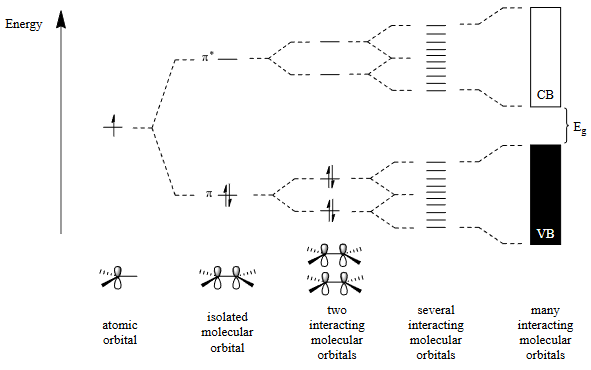
\includegraphics[scale = 0.75]{Bilder/VB-CB.png}
			\caption{}
			\label{VB_CB}
		\end{figure}

	Die Bandlücke E$_\text{g}$ ist dabei der bereich zwischen den beiden Bändern.
	Je größer diese ist desto schlechter leitet der Stoff.
	Da im falle von Leitung ein Elektron vom Valenzband in das Leitungsband übergehen muss.
	Dieser Abstand kann durch Oxidation oder Reduktion verkleinert werden. 
	In Abb. \ref{thiophen} ist dies am Beispiel von thiophen gezeigt dabei sind die beiden dotierten Strukturen gezeigt.
	Im laufe der Oxidation werden elektronen aus dem HOMO entnommen, im falle der Reduktion wird ein elektron in das LUMO aufgenommen.
	Dabei entstehen Ladungen daher ist dieser voregang auch als charging bekannt.
	
		\begin{figure}[H]
			\centering
			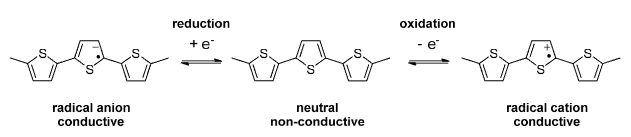
\includegraphics[scale = 0.75]{Bilder/thiophen.png}
			\caption{}
			\label{}
		\end{figure}

	Diese Elektronenabgabe bzw aufnahme kann auch einfluss auf die physischen eigenschaften nehmen wie zB. die Farbe.
	Diese Materialien werden auch elektrochrom genannt. So ist Beispielsweise PDOT im oxidierten Zustand hellblau und wird nach reduktion dunkelblau. 
	Dies lässt sich durch verkleinerung der Bandlücke erklären. Da jeweils immer die Komplementäre Wellenlänge aufgenommen wird ist die aufgenommene energie bei 
	dunkelblau niedriger. Dementsprächend lässt sich eine verkleinereung der Bandlücke erklären. \\

	Das redoxverhalten der Stoffe wird bei der cyclovoltametrie ausgenutzt.
	Hierbei wird im laufe des Experiments wird ein linearer Potentialdurchlauf mit konstanter Scanrate
	(v) in einem bestimmten Potentialfenster durchgeführt. Am Ende des Potentialfensters (Eλ)
	wird die Richtung des Durchlaufs umgekehrt und das Potential linear verringert (mit
	derselben v), bis das Startpotential wieder erreicht ist. 
	Während dieses Potentialdurchlaufs wird der Strom aufgezeichnet und gegen das
	angelegte Potential aufgetragen.
	Die Messung selbst wird über ein drei Elektroden Aufbau ermitteltl. 
	Dabei ist eine der drei Elektroden die Arbeitselektrode, eine die Gegenelektrode und die dritte die Referenzelektrode.
	Zu diesen Elektroden wird die redoxaktive Probe gegeben. 
	Die Referenzelektrode dient hierbei um das Potential zu kontrollieren und um den Start des Potentials festzulegen.
	Dabei werden meist Standard Wasserstoff Elektroden (SHE) oder Silber/Silberchlord Elektroden verwendet.
	In unserem Fall wurde eine Ferrocen/Ferrocenium Elektrode verwendet. 
	%Frage 5 fertig beantworten
	Ein Potentiometer stellt dabei das Potential zwische Arbeits- und Gegenelektrode ein, sodass der Potentialunterschied $\Delta E$ dem eingestellten Wert entspricht.

		\begin{figure}[H]
			\centering
			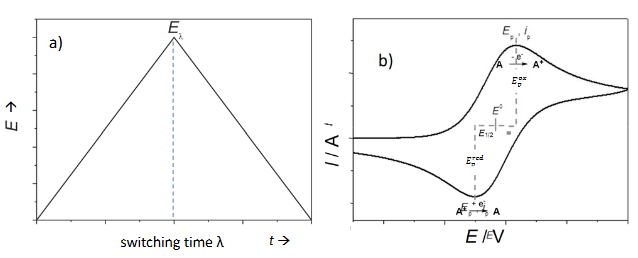
\includegraphics[scale = 0.75]{Bilder/DiagrammeCV.png}
			\caption{}
			\label{CV-Diagramme}
		\end{figure}

	
\section{Durchführung}

	Der Versuch wurde unter Stickstofatmosphäre durchgeführt. Und es wurde eine Pt Platte als Gegenelektrode verwendet.
	Als Referenzelektrode wurde ein mit \ch{AgCl} überzogener Silberdraht verwendet. 
	Als Arbeitselektrode wurde eine Glas überzogene ITO (Indium Tin Oxide) Elektrode verwendet.
	Als Elektrolytlösung wurden \SI{5}{ml} einer 0.1 M \ch{NBu4PF6/MeCN} ( \ch{NBu4PF6}: M = \SI{387.43}{g/mol})-Losung verwendet.
	

\printbibliography

\end{document}